\documentclass[10pt,letterpaper]{article}
 \usepackage[latin1]{inputenc}
 \usepackage[english]{babel}
 \usepackage{amsmath, amssymb, amsfonts}
 \usepackage[total={18cm,23cm}, top=2cm, left=3cm]{geometry}
 \usepackage{graphicx}
 \usepackage{anyfontsize}
 \usepackage{mathptmx}
 
 
 \begin{document}
 	\Large{
 		
 	\begin{center}
 		
 		 {\Huge \bf Problemas de Dise\~no y An\'alisis de Algoritmos}\\
 		 \vspace{1cm}
 		 {\Huge \bf Problema 1: Tareas y Expertos }\\ 
 		 \vspace{1cm}
 		 {\Large \bf Equipo: 3}\\
 		 \vspace{0.5cm}
 		 {\Large \bf Miembros:}\\
 		 {\bf - Laura Brito Guerrero}\\
 		 {\bf - Sheyla Cruz Castro}\\	
 		 {\bf - Rodrigo Garc\'ia G\'omez}\\
 		 
 	\end{center}
 	
 	{\Large \bf Enunciado del Problema:}\\
 	
 	Imagine una cantidad n de tareas, cada una de ellas con determinada complejidad $ci$, que deben ser realizadas. Para hacer esto se cuenta con un grupo $m $ de expertos, caracterizados por sus respectivas capacidades $di$. Se sabe que el experto i-\'esimo puede ejecutar la tarea j-\'esima si $di$ $>=$ $cj$. Cada experto consume un d\'ia en hacer una tarea y ha de recibir por su trabajo una cantidad $ki$ de pesos, que siempre es la misma independientemente del n\'umero de tareas que resuelva. El objetivo en este problema es determinar el menor tiempo posible en que se pueden resolver las $n$ tareas sin pagar m\'as de $k$ pesos. Se asume que las tareas se pueden hacer en cualquier orden y que distintos expertos pueden trabajar al mismo tiempo en sus respectivas tareas.
 	\\ \\
 	
 	\begin{abstract}
 		Primeramente lo atacamos con un algoritmo $fuerza$ $bruta$ exponencial que analiza todas las combinaciones posibles que resultan de distribuir los distintos expertos a tareas, y da la mejor soluci\'on posible. Este algoritmo es ineficiente, por lo cual lo intentamos por otras v\'ias. Una soluci\'on consiste en combinar una $mochila$ para obtener subconjuntos de elementos, con un algoritmo cuadr\'atico para determinar la mejor ganancia; este resulta $n^{3}*k$, tambi\'en de costo exponencial ya que depende del valor de $k$. Una cuarta idea ser\'ia  implementar un algoritmo para, dado un grupo de cient\'ificos fijo v\'alido y las tareas a completar por estos, encontrar la menor cantidad de d\'ias en que pueden lograrlo, de forma polinomial; esta es costosa, pues para determinar dicho grupo tengo que generar todas las combinaciones. Por \'ultimo vimos una idea $greedy$ que consist\'ia en hacer una b\'usqueda binaria sobre un predicado de la forma $no$,$no$...$si$,$si$... buscando el primer si que responda a la menor cantidad de d\'ias que se requieren para realizar las $n$ tareas, con un costo de $n^{2}\log{n}$. \\ \\ \\
 	\end{abstract}
 	
 	{\Large \bf Aclaraci\'on:} \\ \\
 	
 	Para cada uno de los tres problemas se implement\'o un programa $tester$ $generator$ que se encarga de generar de forma aleatoria una inmensa cantidad de ficheros con casos de prueba y un $tester$ con el cual se implementan estos casos con dos o m\'as m\'etodos distintos. De esta forma es posible comprobar con una alt\'isima seguridad la correctitud de un algoritmo a partir de la comparaci\'on de sus resultados con los resultados de otro algoritmo enfocado en la $fuerza$ $bruta$ con una complejidad temporal muy superior, pero cuya correctitud es m\'as evidente. Adem\'as, de esta forma es f\'acil comprobar los casos espec\'ificos en los que determinado algoritmo falla, ayudando as\'i la b\'usqueda y arreglo de errores. Estas demostraciones no producen las demostraciones formales necesarias para la correcta resoluci\'on de los ejercicios, pero son muy \'utiles para dirigir correctamente los esfuerzos, ya sea para demostrar uno en el que se tenga una fuerte convicci\'on de correctitud, o para comprobar los motivos por el que otro es incorrecto. \\ \\
 	
 	
 	
 	{\Large \bf Idea Fuerza Bruta:}\\ \\
 		{\small \bf (brute1)}
 	
 	La idea consiste en generar todas las posibles asignaciones de expertos a tareas. Ser\'ian todas las formas de tomar $n$ tareas del conjunto de tareas(como es condici\'on necesaria que todas las tareas se realicen, se toman todas estas) donde cada una puede tomar $m$ formas distintas,o sea pueden ser realizadas por alguno de los $m$ expertos. De aqu\'i nos quedamos con la combinaci\'on que consuma la menor cantidad de d\'ias entre todas las posibles distribuciones.
 	
 	Inicialmente se esperan tres l\'ineas: la primera con la cantidad de tareas a realizar,la cantidad de expertos y el presupuesto del que se dispone, $n$, $m$, y $k$ respectivamente; luego una segunda con las capacidades de los expertos; y finalmente las complejidades de cada una de las tareas. Una vez que contamos con todos los datos creamos un array con los n\'umeros en el intervalo de $0$ a $n-1$,o sea de tama\~no n,sobre el cual trabajaremos. Por consiguiente generamos todas las posibles distribuciones a trav\'es del m\'etodo $var-rep$.
 	
 	Toda tarea tendr\'a asignada un experto y este ser\'a \'unico pues una tarea solo puede ser realizada una vez. La distribuci\'on admite elementos repetidos, o sea un experto puede realizar m\'as de una tarea. Una vez que se genera una posible distribuci\'on se analiza su factibilidad,de esto se encarga el m\'etodo $analize$. Para ello se comprueba que el experto i-\'esimo asignado a la tarea j-\'esima tenga capacidad mayor o igual que la complejidad de dicha tarea; y se comprueba adem\'as que la suma del dinero que recibe cada experto es menor o igual que el presupuesto con que se cuenta. Una distribuci\'on bajo estas restricciones se considera v\'alida. De todas ellas nos quedamos con la que requiera menor cantidad de d\'ias. La cantidad m\'axima de d\'ias que requiere cada disposici\'on es igual al m\'aximo de la cantidad de tareas que realiza cada experto, pues este requiere de todo un d\'ia para la realizaci\'on de la tarea y estos pueden trabajar simult\'aneamente, luego el que m\'as tareas tenga requerir\'a m\'as d\'ias, y dicha cantidad ser\'a cota m\'axima para el tiempo total requerido. Por \'ultimo nos quedamos con el m\'inimo de los m\'aximos(duraciones m\'aximas de las distintas posibilidades) pues lo que se quiere es minimizar el tiempo de realizaci\'on de las $n$ tareas.
 	
 	La correctitud de esta soluci\'on se sustenta en que se analizan todas las posibilidades, garantizando as\'i que de existir una soluci\'on se va a encontrar y se queda en todo momento con la m\'as \'optima. Este algoritmo es exponencial,genera $m^{n}$ distintas posibilidades, donde  $m$ es el n\'umero de expertos y $n$ el n\'umero de tareas a realizar. Esta soluci\'on es muy ineficiente, se demora considerablemente para peque\~nos valores de la entrada.\\ \\
 	
 	
 	{\Large \bf Idea 2:}\\ \\
 	{\small \bf (calculate-days)}
 	
 	Se implement\'o un algoritmo para, dado un grupo de cient\'ificos fijo v\'alido y las tareas a completar por estos, encontrar la menor cantidad de d\'ias en que pueden lograrlo, de forma polinomial. Se tiene $n$ = la cantidad de tareas y $m$ = la cantidad de cient\'ificos. Primeramente, es necesario ordenar de forma creciente a los cient\'ificos por sus capacidades y las tareas por sus dificultades.
 	
 	La idea consiste en separar a los cient\'ificos por grupos en dependencia de la cantidad de tareas que sean capaces de cumplir. Se mantiene un puntero para cient\'ificos $j$ y otro para tareas $i$. Se avanza el puntero $i$ por las tareas hasta que el cient\'ifico $j$ no sea capaz de cumplir la tarea $i$, entonces se agrega al nuevo grupo al cient\'ifico $j$ y a todos los cient\'ificos siguientes que tampoco sean capaces de cumplir dicha tarea, avanzando el puntero $j$. Los grupos llevar\'an constancia de la cantidad de tareas que pueden cumplir y la cantidad de cient\'ificos que poseen. La conformaci\'on de los grupos se realiza en tiempo lineal $m + n$ pues es evidente que se pasa s\'olo una vez por cada tarea y una por cada cient\'ificos.
 	
 	Todas las tareas realizadas por un grupo se podr\'an realizar tambi\'en con los grupos superiores, por tanto se buscar\'a repartir las tareas de forma que si el grupo $i$ realiza sus tareas en un tiempo superior al grupo $i + 1$, este aumente sus d\'ias en uno para ayudar al grupo $i$. Este proceso se repetir\'a cada vez que el grupo $i$ tenga mayor tiempo que el $i + 1$. Al realizar esto para todos los grupos, cuando el algoritmo termine, entonces en el \'ultimo grupo tendr\'a la mayor cantidad de d\'ias entre todos los dem\'as, y por tanto, como todos los dem\'as grupos finalizar\'an sus tareas en un tiempo menor o igual que \'el, esta ser\'a la cantidad de d\'ias a retornar. Este retorno tendr\'a la cantidad m\'inima de d\'ias de trabajo, puesto que los d\'ias de los grupos superiores aumentar\'an un d\'ia a la vez, mientras que los de grupos inferiores disminuir\'an en uno o m\'as d\'ias, por tanto, si el grupo $i$ se completa en m\'as d\'ias que el $i + 1$, la cantidad de d\'ias que se le aumentan a este, no ser\'a mayor que la que ten\'ia el $i$ antes de disminuirle.
 	
 	A partir de este momento, solo se trabajar\'a con la lista de grupos de cient\'ificos reci\'en formada. El ciclo principal iterar\'a por dicha lista de forma descendiente, a partir de la \'ultima posici\'on (recordemos que esta lista est\'a ordenada). Primeramente, en cada iteraci\'on (siendo la iteraci\'on $i$, que se est\'a analizando el grupo $n - i$), si la cantidad de tareas es mayor que la cantidad de cient\'ificos, se divide tareas entre cient\'ificos y se guarda en una variable $q$ (esto representa la cantidad de d\'ias necesaria para que el grupo termine sus tareas), en caso de haber resto se incrementa $q$ en uno y en una variable $r$ se almacena la diferencia entre los cient\'ificos del grupo y dicho resto (esto representa el sobrante de tareas del grupo para realizar las suyas en la cantidad de d\'ias $q$, o sea, si el grupo tiene $2$ cient\'ificos y $5$ tareas, en $3$ d\'ias realiza sus tareas, y tiene uno de resto para almacenar). Adem\'as, si el grupo bajo an\'alisis actual realiza sus tareas en una cantidad de d\'ias $q$ mayor que el grupo inmediatamente superior, le pedir\'a a este una ayuda, incrementando en el grupo superior una variable que almacena las ayudas a prestar al grupo inferior; luego es necesario recalcular $q$ y $r$ del grupo actual pero retirando una cantidad de tareas similar a la cantidad de ayudas de su grupo superior multiplicada por la cantidad de cient\'ificos de este, de lo cual se encarga el ciclo principal, que se repite siempre que ocurra una $pedida$ $de$ $ayuda$. Si la cantidad de tareas es menor que la cantidad de cient\'ificos, el proceso es similar, con la diferencia de que en lugar de hacer un divisi\'on, en $q$ se almacenar\'a $1$, y en $r$, la substracci\'on de los cient\'ificos por las tareas (si hay $5$ cient\'ificos y $3$ tareas, se cumplen en un d\'ia y se guarda $2$ de resto para quitarle tareas al grupo inmediatamente menor) . Al terminar el ciclo principal, la soluci\'on quedar\'a representada en la cantidad de d\'ias $q$ m\'as la cantidad de ayudas prestadas por el grupo de la \'ultima posici\'on de la lista (el de las mayores capacidades).\\ \\
 	
 	
 	{\Large \bf Idea 3:}\\ \\
 	{\small \bf (knapsack)}
 	
 	Otra soluci\'on un poco m\'as eficiente para este problema es combinarlo con una $mochila$ y luego aplicarle un algoritmo cuadr\'atico que garantice obtener la mejor ganancia, sobre los elementos que se encuentran escogidos en la $mochila$, para as\'i garantizar obtener la mayor ganancia. Esta idea se lleva a cabo de la siguiente manera: inicialmente tenemos una mochila de peso $k$, el cual es el presupuesto destinado para la realizaci\'on de las tareas. Como cada experto tiene una ganancia $ki$ independientemente de la cantidad de proyectos que realice, esta misma representar\'ia los pesos correspondientes a cada uno. 
 	
 	Como este algoritmo me garantiza que en cada momento exista una repartici\'on v\'alida de expertos, tenemos que ahora distribuir las tareas entre ellos tal que se cumpla que todas las tareas se tomen y de esta forma hallar la mejor combinaci\'on tal que el m\'aximo de las tareas entre los expertos sea m\'inima. Esta combinaci\'on asignada resultar\'a la ganancia de esta repartici\'on, y en cada elecci\'on de expertos ir guardando este m\'aximo de tareas con la intenci\'on de que la ganancia se minimice. Por lo que variaremos la salida del algoritmo $mochila$ est\'andar, puesto que en vez de buscar la ganancia m\'axima (la cantidad de d\'ias m\'aximos) se hallar\'a la m\'inima. 
 	
 	Para hallar la combinaci\'on de las tareas por los expertos de manera eficiente se realiz\'a el siguiente algoritmo: se tiene un arreglo de $n$ tareas con sus respectivas complejidades, y se tienen $mk$ expertos escogidos. Las tareas estar\'an ordenadas decrecientemente por complejidad, y se ordenar\'an por capacidad en orden decreciente a los expertos escogidos. Se recorrer\'an las tareas en ese orden intentando otorg\'arselas a los distintos expertos, de manera tal que todos los expertos tengan tareas, y siempre se tratar\'a de otorgar la menor cantidad de tareas por experto. Esto se realiza en dos ciclos anidados siempre analizando las tareas a entregar. \\ \\
 	
 	{\Large \bf Idea 4:}\\ \\
 	{\small \bf (greedy)}
 	
 	Esta idea se basa en hacer una b\'usqueda binaria sobre un predicado de la forma \\
 	$no$,$no$...$si$,$si$... buscando el primer s\'i que responda a la menor cantidad de d\'ias que se requieren para realizar las $n$ tareas. El predicado tiene esta forma pues si se pueden realizar las $n$ tareas en una cantidad $i$ de d\'ias, con $i$ $<=$ $n$, en una cantidad mayor tambi\'en se podr\'a hacer. \\ 
 	
 	Sea la funci\'on definida como sigue a continuaci\'on:\\
 	
\begin{equation}
 	f(x) = \left\{ \begin{array}{lcc}
 	0 & si &  imposible \\
 	1 & si &  posible\\
 	\end{array}  \right
\end{equation}
 	
 	Donde $posible$ significa que se pueden hacer las tareas en $x$ cantidad de d\'ias e $imposible$ que no se pueden hacer en dicha cantidad.
 	
 	Se puede ver que esta funci\'on es un predicado que aplicado sobre el intervalo $[1, n]$, siendo $n$ la cantidad total de tareas a realizar para una entrada del problema, se obtiene una secuencia de resultados $[0,0,0,...,1,1,...,1]$. Se aprecia adem\'as que la secuencia de resultados es bimodal. Analizando el anterior razonamiento se tiene que demostrar que $f(x) = 1 => f(x + 1) = 1 $ o sea una vez que se puedan realizar las $n$ tareas en $x$ cantidad de d\'ias, se pueden realizar en una cantidad de d\'ias mayor.\\
 	
 	Intentemos demostrarlo por v\'ia directa:\\
 	Se tiene que se pueden realizar las $n$ tareas en $x$ cantidad de d\'ias, veamos si es posible realizarlas en $x + 1$ d\'ias, para esto solo tenemos que asignarle $x + 1$ tareas al experto de mayor capacidad entre los expertos que participan en la realizaci\'on de las tareas, estas tareas deben ser las m\'as costosas para asegurar la realizaci\'on de todas, esto es posible hacerlo pues si el que m\'as capacidad tiene entre ellos no puede hacerlas, nadie podr\'a, entonces no se podr\'ia haber hecho en $x$ d\'ias, y adem\'as el presupuesto ser\'a suficiente, pues no se est\'a variando ning\'un experto, se est\'an usando los que ya participaban, luego el costo final ser\'a el mismo que para $x$ d\'ias resolv\'ia. Las tareas que este experto de presupuesto m\'aximo hac\'ia, que son una cantidad menor que $x+1$, pues sino la cantidad de d\'ias fuera esta, se le dan a los expertos de los cuales se quitaron las tareas que fueron a parar al experto de costo m\'aximo, esto se puede hacer, pues si se le quito una tarea de mayor complejidad ser\'a entonces capaz de hacer una de menor, y adem\'as su cantidad de tareas se mantendr\'a igual, pues se le adicionan la misma cantidad que se le restan. El presupuesto no se ve afectado, pues los intercambios se realizan entre los expertos que ya participaban, por tanto este no var\'ia. La cantidad de tareas m\'aximas que realizar\'a alg\'un experto haciendo esta repartici\'on ser\'a $x+1$, pues anteriormente era $x$, y de las que se modificaron solo una adquiri\'o la cantidad $x+1$, el resto se mantiene igual. Por tanto se pueden realizar las $n$ tareas en $x+1$ cantidad de d\'ias a partir de que era posible con $x$ cantidad.
 	
 	Como lo que se quiere es minimizar la cantidad de d\'ias lo que se busca es el primer $si$. Esto se puede hacer en $\log n$, el problema consiste en encontrar el experto capaz de realizar una cantidad de tareas $i$ que coincide con la cantidad d d\'ias en cuesti\'on, esta misma cantidad ser\'ia igual al m\'aximo de tareas que se le puede asignar a un experto de modo que se puedan repartir el resto de las tareas entre los expertos que quedan, este experto ya no estar\'ia disponible pues si a \'el se le pudiesen asignar m\'as tareas aumentar\'ia la cantidad de d\'ias. 
 	
 	Se ordenan las tareas decrecientemente por complejidad. Se recorren en dicho orden, intentando asignarle el subconjunto de tama\~no $m$, donde $m$ es la cantidad de d\'ias que se determina en la b\'usqueda binaria, al experto que menos costo tiene(o sea al que menos cobra por realizar una tarea) entre el todos aquellos capaces de realizar todas las tareas del subconjunto. Con comprobar si el experto es capaz de realizar la tarea m\'as costosa es suficiente, pues si puede hacer esta ser\'a capaz de realizar el resto. De nadie poder hacer esta tarea se retorna no inmediatamente pues habr\'a una tarea que nadie podr\'a realizar, lo cual no es posible. Se comprueba adem\'as que lo que cobra este experto sumado al monto total que se va acumulando en cada asignaci\'on(variable $mont$) sea menor que el presupuesto, de esto no suceder se retorna $False$ inmediatamente, lo cual supone un $no$ para mi predicado, pues de no poder el de menor costo de todos los que pueden realizarla, no se podr\'a pagar tampoco ning\'un otro experto de los que son capaces de hacerla(o sea no puedo acudir a ning\'un otro experto que cobre menos, pues este no ser\'a capaz de hacerla, sino se encontrara en mi conjunto de candidatos), pues se escogi\'o el que menos cobraba. Una vez asignada esa cantidad de tareas de eliminan de la lista de tareas, al igual que el experto que las realiz\'o, pues estas solo pueden ser realizadas una sola vez, y el experto en cuesti\'on no puede recibir m\'as tareas pues sino la cantidad de dias m\'inimos aumentar\'ia. Se contin\'ua el recorrido repitiendo el procedimiento anterior, si se consiguen asignar todas, es un $si$ de mi predicado, pues todas las tareas se van a realizar, la cantidad de d\'ias va a ser $m$, pues ning\'un experto recibe m\'as de esa cantidad, y todos reciben tareas que pueden realizar y lo que cobran est\'a por debajo del presupuesto.\\ \\
 	
 	Esta idea es greedy, por lo tanto es necesario demostrar su correctitud. \\
 	\textit{Demostraci\'on} \\
 	Sean las soluciones
 	\begin{center}
 	\textit{Opt = $\{ Y_{1}, Y_{2}, . . . , Y_{n} \}$, $Y_{i}$ vectores de la soluci\'on \'optima Opt y \\
 	G = $\{ X_{1}, X_{2}, . . . , X_{n} \}$, $X_{i}$ vectores de la soluci\'on greedy G.}
 	\end{center}
 	Ambas soluciones tienen cardinalidad $n$ ya que estos vectores representan a los expertos que realizan la tarea $i$. Se ha de destacar que las tareas se ordenan por complejidad de manera decreciente, por tanto en la posici\'on i-\'esima de la soluci\'on se recoge el experto que resolvi\'o la tarea i-\'esima en orden decreciente. \\
 	\begin{center}
 	\textit{$Z_{i}$ resuelve la tarea de complejidad $c_{i}$, $\forall$ $Z_{i} \in \{ X_{i}, Y_{i} \}$} \\
 	\end{center}
 		Est\'a claro que pueden existir vectores iguales, ya que si las tareas $c_{i_{1}}, c_{i_{2}}, . . ., c_{i_{k}}$ las realiza el mismo experto entonces $Z_{i_{1}}, Z_{i_{2}}, . . ., Z_{i_{k}}$. \\
 	
 
 	
 	Primeramente se enunciar\'a un lema muy \'util en la demostraci\'on. \\ \\
 	
 	 		\begin{figure}
 	 			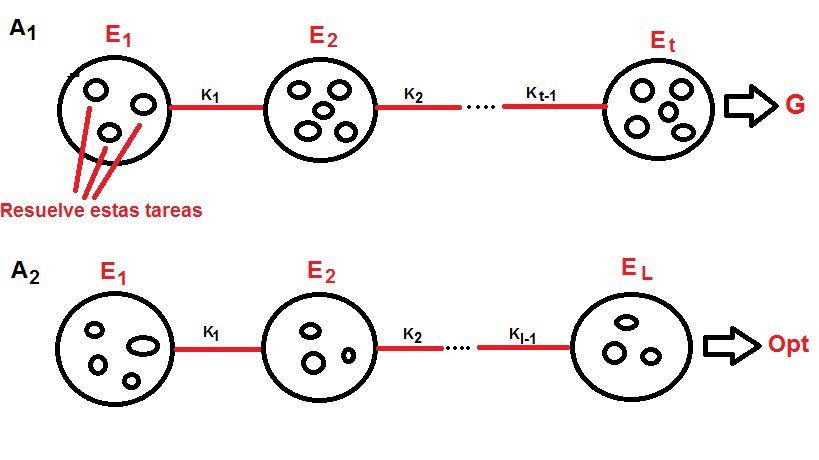
\includegraphics[width=10cm]{mst.png}
 	 			\caption{\'Arboles que representan a las soluciones $G$ y $Opt$, donde los v\'ertices representan al experto con las tareas que realiza, las aristas representa el costo de los expertos, la arista $i$ es el costo del experto $i$, y el \'ultimo experto se enlaza con un nodo fictisio, para poder asignarle el costo al mismo}
 	 		\end{figure}
 	
 	\textit{Lema 1:} \\
 	Si se observa la soluc\'ion del algoritmo greedy $G$ como $A_{1}$(figura 1), entonces $A_{1}$ es un MST (Arbol abarcador de costo m\'inimo). \\
 	\textit{Demostraci\'on} \\
 	La correctitud de la b\'usqueda del MST, en el algoritmo de Kruskall, se demostr\'o en conferencia. \\
 	\textit{Lema 1.1: $A_{1}$ es un \'arbol.}  \\
 	\textit{Demostraci\'on:} De la forma que se construye $A_{1}$ se tiene que \'el es un camino simple de longitud $t$. No existen ciclos en \'el puesto que a los expertos escogidos en el algoritmo se le asignan las tareas, y estos constituyen los nodos (v\'ertices), no habr\'a una arista que comunique el vertice $E_{i}$ con alguno de los anteriores utilizado en el camino, y esto no sucede porque significa que existe m\'as de un experto realizando al menos una tarea en com\'un, y esto no sucede porque a la vez que se asigne una tarea, la misma no se vuelve a analizar. Como $A_{1}$ es un camino simple entonces $A_{1}$ es un \'arbol, donde los nodos extremos tienen degree 1 y los interiores degree 2. \\ \\
 	Supongamos que $A_{1}$ no es un MST. Entonces sea $T$ un MST de $G$ tal que $w(T) \leq k$. \\
 	Como $A_{1}$ no es un MST se cumple que $W(T) \leq w(A_{1}) \leq k$. \\
 	Si analizamos la idea del algoritmo greedy es f\'acil de percatar que al organizar las tareas por complejidades y a los expertos por capacidades de maner decreciente, se tiene un an\'alisis de subconjuntos. Esto se explica de la siguiente forma, al escoger las $x$ tareas que se van a asignar, se escogen un grupo de expertos capaces de ejecutarlas, pero de todos ellos se escoger\'a el que menos costo tenga (menos le paguen). \\
 	Recorramos el camino simple de $T$ y $A_{1}$ por paso. Existe al menos una arista tal que $w(e_{1}) > w(e_{2})$, donde $e_{1} \in A_{1}$ y $e_{2} \in T$. Estas aristas existen puesto que $A_{1}$ no es un MST. \\
 	Esto significa que para este conjunto de tareas se escogi\'o un experto en $A_{1}$ con presupuesto $>$ que el de $T$. Hasta el momento los expertos que se escogen en $T$ son los mismos que tiene $A_{1}$. En toda iteraci\'on $A_{1}$ analiza los expertos de mayores capacidades: \\
 	sea $E_{i}$ con $k_{i}$ = $e_{1}$, $E_{i} \in A_{1}$ y $E_{j}$ con $k_{j}$ = $e_{2}$, $E_{j} \in T$ donde $k_{i} > k_{j}$. \\
 	Se toman tres casos: \\ \\
 	\textit{1: $d_{i} > d_{j}$} \\
 	Es trivial percatarse que este subconjunto $i$ tiene el bloque de mayores capacidades sin analizar, pero los $i- 1$ subconjuntos anteriores tienen mayor capacidad que \'el, ya que las tareas est\'an ordenadas decrecientemente por complejidad y separadas en intervalos de a lo sumo cardinalidad $x$. Por lo que se ramifucan dos subcasos: \\
 	\textit{1.1: $d_{i} > d_{k} \forall k \in N, 0 \leq k \leq i - 1, d_{k} \in A_{1}$.} \\
 	Si esto ocurre es porque en an\'alisis anteriores se decidi\'o tomar un experto con menor capacidad pero capaz de realizar las tareas del bloque k. \\
 	\textit{1.1.1: $d_{k} \geq d_{j}$} \\
 	Supongamos que $d_{j}$ no puede con las tareas de $d_{i}$. Significa que el m\'aximo de las complejidades tomadas por $E_[i]$ es mayor que $d_[j]$. Si esto ocurre tratemos de colocar la tarea con complejidad m\'axima de $E_{i}$ (llam\'emosle $c^{'}$) para alguno de los anteriores. Es imposible lo anterior porque los expertos escogidos tienen asignadas $x$ taraes y no le caben m\'as. \\
 	Como $T$ est\'a ordenado igualmente por capacidades y complejidades, se tiene que $d_{j}$ no es v\'alido para sus tareas asignadas, lo cual es una contradicci\'on porque $T$ es v\'alido. Por lo tanto $d_{j}$ puede con las tareas de $d_{i}$, nuevamente contradicci\'on aqu\'i, ya que $A_{1}$ hubiera escogido a $E_{j}$ y no a $E_[i]$. \\
 	\textit{1.1.2: $d_{k} \leq d_{j}$ } \\
 	Si $d_{k}$ pudo hacer tareas de mayor complejidad entonces $d_[j]$ puede hacer cualquier otro bloque posterior de tareas, lo cual es un contradicci\'on ya que $A_{1}$ tomar\'ia a $E_{j}$ en lugar de $E_{i}$. \\
 	\textit{1.2: Si $d_{i}$ es el mayor en el paso $i$ } \\
 	Si esto sucede significa que en $T$ existe un experto con capacidad $d_{j}$ que realiza las mismas tareas que $d_{i}$, donde $d_{j} < d_{i}$, como $T$ es v\'alido entonces se genera una contradicci\'on, ya que $A_{1}$ tomar\'ia a $E_{j}$, el cual es capaz de resolver ese bloque de tareas con un presupuesto menor. \\ \\   
 	\textit{2: $d{i} < d_{j}$} \\
 	Significa que si el subconjunto de tareas tomados de cardinalidad a lo sumo $x$, que tiene las mayores capacidades despu\'es del an\'alisis de los $i - 1$ subconjuntos anteriores, se puede realizar con un experto de capacidad menor o igual que otro que tenga mayor capacidad y menor presupuesto, entonces $d_{j}$ tambi\'en puede ejecutar ese subconjunto de tareas. Como en $A_{1}$ se toman los expertos con capacidad v\'alida y menor presupuesto (Contradicci\'on: $A_{1}$ tomar\'ia $E_{j}$ desde un principio). \\ \\
 	\textit{3: $d_{i} = d_{j}$} \\
 	 Directamente se genera una contradicci\'on, ya que $A_{1}$ elige el de menor presupuesto, o sea, $E_{j}$. \\ \\
 	 Por tanto, tras una cantidad finita de pasos se demuestra que $A_{1}$ es un MST. \\ \\
 	 
 	 Tomemos la primera posici\'on $i$ tal que $Y_{i} \neq X_{i}$. Tengamos presente que un bloque completo de $G$ es el mismo experto($x$ expertos). Se tienen dos casos: \\
 	 \textit{1: $X_{i}.k \leq Y_{i}.k$} \\
 	 Como $X_{i} \in V(A_{1})$, entonces por $Lema 1$ se cumple que $Y_{i}.k > X_{i}.k$, por lo que $Y_{i}.k - X_{i}.k$ es el excedente de presupuesto que tiene $Opt$ con respecto a $G$. La idea es quitar este excedente a otros de $k$ en adelante de manera que siga quedando factible.\\
 	 Esto es v\'alido porque como las tareas est\'an ordenadas decrecientemente por complejidad entonces si se le asigna el vector $Y_{i} = X_{i}$ quedando el $Opt$ factible ya que si $X_{i}$ pudo realizar esta tarea con menor capacidad entonces se cambian y disminuye el presupuesto asignado al excedente de este paso. De esta manera tambi\'en se garantiza que el predicado sea v\'alido y no exista un experto con m\'as de $x$ tareas. \\
 	 \textit{2: $X_{i}.k > Y_{i}.k$} \\
 	 Si esto ocurre se cumple que $Y_{i}$ fue escogido necesariamente antes por $G$ (por ser $A_{1}$ MST), de lo contrario $Y_{i} \in G$ por propiedad de $A_{1}$, por tanto $Y_{i}$ no estaba disponible para la tarea. Para no llegar a una contradicci\'on con respecto a $w(A_{1})$ ya que es el menor costo posible de tomar. Como en las anteriores iteraciones donde se cumpl\'ia el caso 1 y realiz\'abamos las modificaciones con el objetivo de disminuir $w(A_{2})$. \\
 	 Como $w(A_{1}) \leq w(A_{2})$ entonces es v\'alido asignar $Y_{i} = x_{i}$, ya que el presupuesto que se quita anteriormente se va agregando de la menor manera posiblegarantizando que no ocurra: $w(A_{2}) < w(A_{1})$ lo cual es un absurdo, por ser $A_{1}$ MST. \\
 	 Por  lo tanto se le agrega a $w(A_{2})$ el monto de $X_{i}.k - Y_{i}.k$. \\ \\
 	 Tras una cantidad finita de pasos tenemos que $w(A_{1}) = w(A_{2})$, equivalente a $G = Opt$ lo cual demuestra que $G$ tambi\'en es una soluci\'on \'optima. \\ \\
 	
 	
 	Este algoritmo tiene una complejidad polinomial, realiza $n^{2} \log{n}$ operaciones, la b\'usqueda binaria en $\log{n}$ buscando el primer $si$, y luego para responder el predicado, hace en el peor de los casos una pasada por todas las tareas, y por cada una de estas recorre los $m$ expertos buscando el de menor costo. Esto ser\'ia $m*n$, luego de no ser iguales, entonces uno es mayor que otro, sea el mayor $m$ sin p\'erdida de generalidad, se puede decir que este es $n+k$, con $k$ $<$ $n$, luego esto es $n^{2}+k$, qued\'andonos con el m\'aximo se tiene entonces $n^{2} \log{n}$.  
 	
 	

}
 	
 \end{document}